\begin{frame}{Konstrukcija pravokotnice}
 \begin{columns}
    \begin{column}{0.55\textwidth}
	\begin{itemize}
		\item Dana sta premica \(p\) in točka \(T\).
		\onslide<2-7>{\item Nariši lok \(k\) s središčem v \(T\).}
		\onslide<3-7>{\item Lok \(k\) seče premico \(p\) v točkah \(A\) in \(B\).}
		\onslide<4-7>{\item Nariši lok \(m\) s središčem v \(A\).}
		\onslide<5-7>{\item Nariši lok \(n\) s središčem v \(B\) in z enakim polmerom.}
		\onslide<6-7>{\item Loka se sečeta v točki \(C\).}
		\onslide<7>{\item Premica \(TC\) je pravokotna na \(p\).}
	\end{itemize}
    \end{column}
    \begin{column}{0.45\textwidth}
	\only<1>{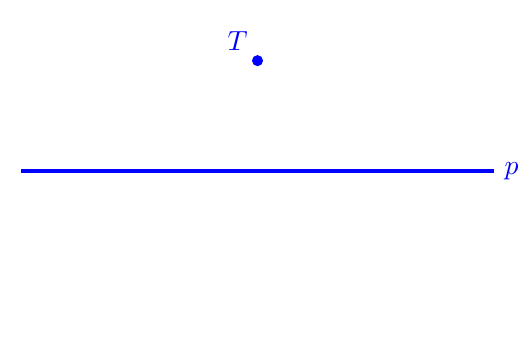
\includegraphics[width=50mm]{slike/fig-1.png}}%
	\only<2>{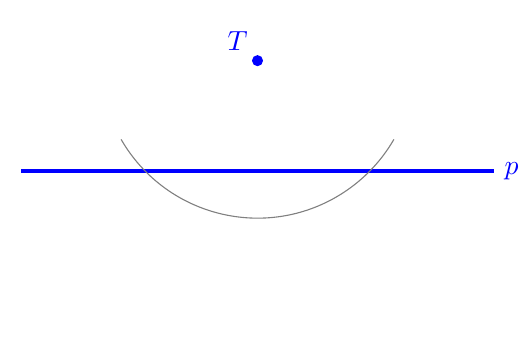
\includegraphics[width=50mm]{slike/fig-2.png}}%
	\only<3>{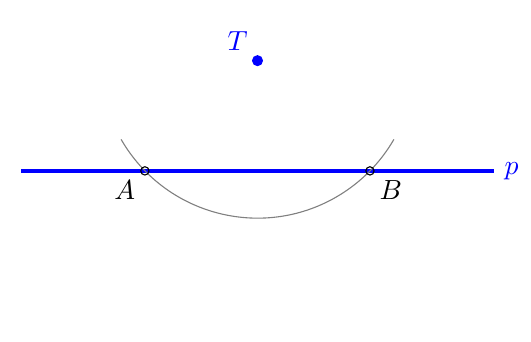
\includegraphics[width=50mm]{slike/fig-3.png}}%
	\only<4>{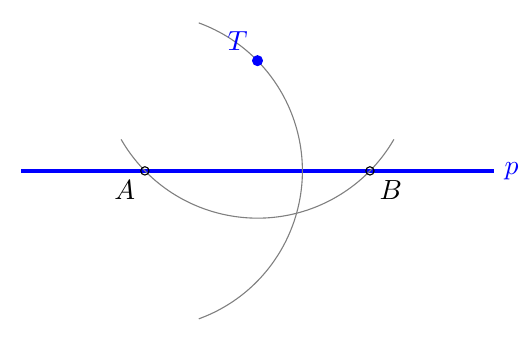
\includegraphics[width=50mm]{slike/fig-4.png}}%
	\only<5>{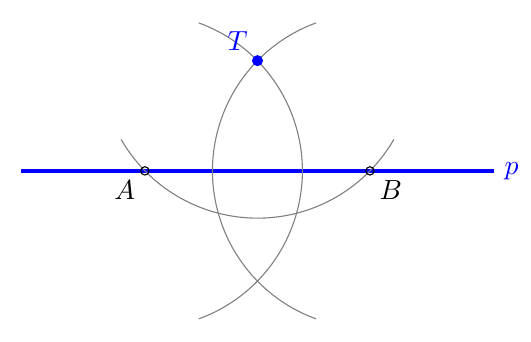
\includegraphics[width=50mm]{slike/fig-5.png}}%
	\only<6>{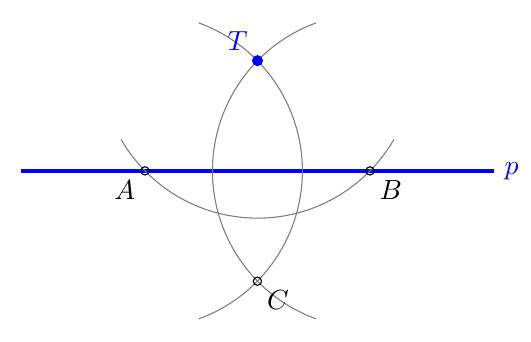
\includegraphics[width=50mm]{slike/fig-6.png}}%
	\only<7>{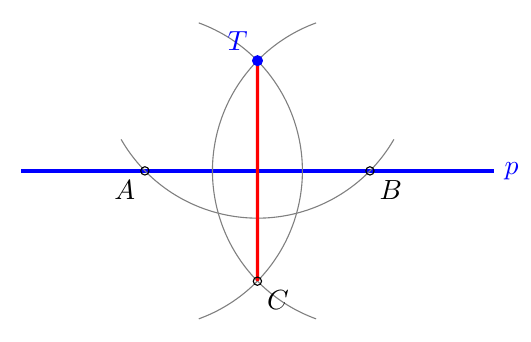
\includegraphics[width=50mm]{slike/fig-7.png}}%
	\end{column}
\end{columns}
\end{frame}
